\documentclass{article}

\usepackage[french]{babel}
\usepackage[utf8]{inputenc}
\usepackage{lipsum}
\usepackage{amsmath, amssymb, amsthm, graphicx}
\usepackage{tikz}
\usepackage{multicol}
\usepackage[hidelinks]{hyperref}
\usepackage{cite}
\usepackage{caption}
\captionsetup{font=footnotesize}
\usepackage{multirow}
\usepackage{adjustbox}
\usepackage{listings}
\usepackage{float}
\setlength{\parindent}{0pt}
\newtheorem{theorem}{Théorème}

%%%%%%%%%%%%%%%% Lengths %%%%%%%%%%%%%%%%
\setlength{\textwidth}{16.5cm}
\setlength{\evensidemargin}{-0.5cm}
\setlength{\oddsidemargin}{-0.5cm}
\setlength{\topmargin}{-1.5cm}
\setlength{\textheight}{23cm}

%%%%%%%%%%%%%%%% Variables %%%%%%%%%%%%%%%%
\def\projet{2}
\def\titre{Compression d’image à travers la factorisation SVD}
\def\groupe{4}
\def\equipe{4}
\def\responsible{Antonin Cochon}
\def\secretary{Mano Domingo}
\def\others{Matheline Chevalier, Melissa Colin, Numa Guiot}

%%%%%%%%%%%%%%%% Image Path %%%%%%%%%%%%%%%%
\graphicspath{{./img/}}

\begin{document}

%%%%%%%%%%%%%%%% Header %%%%%%%%%%%%%%%%
\begin{minipage}{0.98\textwidth}
  \vskip 0mm
    { \begin{tabular}{p{7.5cm}}
      {\bfseries \sffamily
        Projet \projet} \\ 
      {\itshape \titre}
    \end{tabular}}
  \hfill 
  \fbox{\begin{tabular}{l}
      {~\hfill \bfseries \sffamily Groupe \groupe\ - Équipe \equipe
        \hfill~} \\[2mm] 
      Responsable : \responsible \\
      Secrétaire : \secretary \\
      Codeurs : \others
    \end{tabular}}
  \vskip 4mm ~

  ~~~\parbox{0.95\textwidth}{\small \textit{Résumé~:} \sffamily Ce rapport présente un algorithme de compression d'images basé sur la factorisation SVD. Nous avons développé des algorithmes de bidiagonalisation et de décomposition QR pour obtenir la SVD de l'image. Nous avons expérimenté différentes méthodes de compression d'images et avons évalué la qualité de la compression, le gain de place obtenu et les performances de nos algorithmes.}
  \vskip 1mm ~
\end{minipage}



% \section{Introduction}

% \subsection{Contexte}
% La compression d'images est essentielle pour réduire l'espace de stockage et améliorer la transmission des données. La factorisation SVD est une technique puissante pour atteindre cet objectif en réduisant le rang de la matrice représentant l'image.

% \subsection{Motivation}
% Ce projet vise à explorer les techniques de compression d'images en utilisant la factorisation SVD. Nous avons choisi cette méthode pour son efficacité et sa capacité à préserver la qualité visuelle des images compressées.

\section{Méthodologie}
Dans ce travail, nous avons développé un algorithme de compression d'images utilisant la factorisation SVD.\\
Pour cela, nous avons réalisé un algorithme permettant de transformer une matrice en une matrice bidiagonale. Puis, nous avons développé un autre permettant de la transformer en une matrice diagonale de valeurs singulières nécessaires au dernier algorithme qui permet de compresser l'image.\\
Pour réaliser ces algorithmes, nous avons aussi eu besoin de développer les outils nécessaires aux transformations de Householder et à la décomposition QR.\\ \\
L'ensemble des expérimentations a été réalisé sur un système avec un processeur AMD Ryzen 7 7840HS et 64 Go de RAM. %et une carte graphique NVIDIA RTX A500 Laptop GPU.

\subsection{Bidiagonalisations}
\label{sec:bidiagonalisation}
La première étape du SVD est la transformation de la matrice en une matrice bidiagonale, pour ce faire, nous avons réalisé un algorithme de bidiagonalisation basé sur les matrices de Householder. Dans le cadre de ce travail, les matrices de Householder sont un outil puissant. Nous allons donc dans un premier temps aborder la méthode de calcul de ces matrices.\\ \\
\textbf{Matrices de Householder}\\
On cherche à définir une matrice de Householder $H$ telle que $HV = U$ et $HU = V$ où $U$ et $V$ sont des vecteurs de même norme à partir du vecteur $N$ tel que $H = I - 2 \times N \cdot N^T$. La figure \ref{fig:householder} montre cette transformation des vecteurs $U$, $V$, et $H(U)$ dans un espace 3D.
\begin{figure}[H]
\centering
\begin{minipage}{0.35\textwidth}
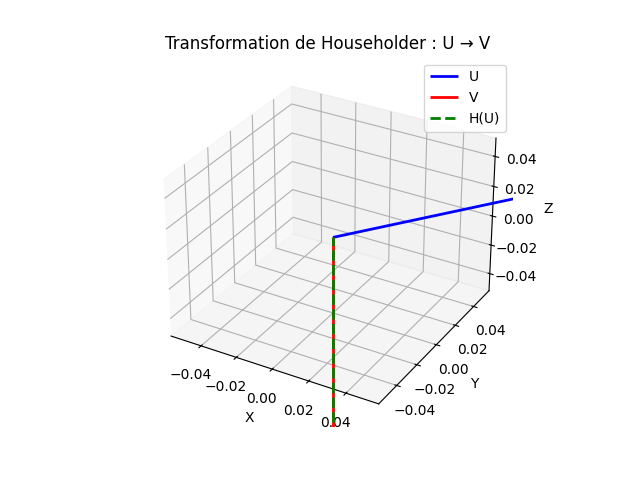
\includegraphics[width=\textwidth, trim=3cm 0 2.5cm 0, clip]{householder_transformation.png}
\caption{Transformation de Householder : $U$ vers $V$.}% Le vecteur bleu est $U$, le vecteur rouge est $V$, et le vecteur vert est $H(U)$, résultat de la transformation.}
\label{fig:householder}
\end{minipage}
\hfill
\begin{minipage}{0.62\textwidth}
Pour trouver $N$ à partir de $U$ et $V$, on calcule tout d'abord sa direction $W = U - V$. Puis on la normalise pour obtenir $N = \frac{W}{\|W\|}$.\\ \\
Pour appliquer la transformation de Householder à un vecteur $X$ efficacement, nous recalculons la transformation de Householder à partir de $N$ plutôt qu'en utilisant une matrice $H$ pré-calculée. Cette méthode permet une meilleure efficacité mémoire car la représentation vectorielle de $N$ est beaucoup plus compacte que $H$. \\
Calculer à partir de $N$ permet aussi d'améliorer les performances, évitant la multiplication par une matrice complète. On utilise alors la formule $H(X) = X - 2 \times N \cdot (N^T \cdot X)$. \\
Ainsi, pour l'appliquer à une matrice, on applique la transformation à chaque colonne (ou ligne) de la matrice par la formule $H(X) = X - 2 \cdot ((N \cdot N^T) \cdot X)$  (ou $H(X) = X - 2 \times (X \cdot (N \cdot N^T))$ pour les lignes).

\end{minipage}
\end{figure}
La transformation sur un vecteur utilise le produit scalaire calculé en $O(n)$, ce qui est optimal pour un vecteur de taille $n$. Sa complexité globale est donc linéaire. Pour l'application à une matrice, le système est le même sur chaque colonne (ou ligne) de celle-ci. La complexité est donc toujours linéaire en $O(n \cdot m)$, où $n$ est le nombre de lignes et $m$ le nombre de colonnes de la matrice.\\
En comparaison avec un produit matriciel usuel par $H$, qui aurait une complexité de $O(n^3)$ (ou $O(n^{2.81})$ avec l'algorithme de Strassen), les méthodes utilisées ici sont beaucoup plus efficaces.\\
Pour confirmer cette différence de performance, nous avons généré des matrices aléatoires de taille \( n \times n \), avec \( n \) variant de 4 à 100, et avons calculé le temps d'exécution ainsi que l'erreur relative moyenne pour chaque taille de matrice. L'erreur relative est calculée selon la formule \(\frac{\| \mathbf{R}_{\text{référence}} - \mathbf{R}_{\text{méthode}} \|}{\| \mathbf{R}_{\text{référence}} \| + \epsilon}\) où \( \mathbf{R}_{\text{référence}} \) est le produit de référence \textit{np.dot(H, X)}, \( \mathbf{R}_{\text{méthode}} \) est le résultat obtenu par la méthode testée, et \( \epsilon \) la précision machine.\\ \\
\textbf{Bidiagonalisation}\\
Ainsi, notre algorithme de bidiagonalisation est basé sur les matrices de Householder qui multiplient à gauche et à droite la matrice d'entrée $A$ pour annuler les éléments.\\ \\
L'algorithme initialise $Q_{\text{left}}$ et $Q_{\text{right}}$ par des matrices identités et $BD$ par une copie de $A$.\\
Pour chaque colonne $i$, on construit deux matrices de Householder $Q_1$ et $Q_2$ qui annulent les éléments sous et à droite du premier élément de la colonne $i$ respectivement. On met à jour les matrices $Q_{\text{left}}$ et $BD$ en multipliant par $Q_1$ et on met à jour les matrices $Q_{\text{right}}$ et $BD$ en multipliant par $Q_2$.\\
À chaque itération, on vérifie que $Q_{\text{left}} \times BD \times Q_{\text{right}}$ est égale à la matrice de départ $A$ à une erreur machine près, proportionnellement à la taille de la matrice. 

\subsection{Diagonalisation}
Après avoir transformé la matrice $A$ en une matrice bidiagonale $BD$ (voir section~\ref{sec:bidiagonalisation}), nous appliquons l'algorithme QR de façon itérative pour obtenir les matrices $U$, $S$ et $V$ où $S$ est une matrice diagonale de valeurs singulières et $U$ et $V$ sont des matrices orthogonales.\\
L'algorithme initialise tout d'abord $U$ et $V$ comme matrices identités et $S$ comme la matrice bidiagonale obtenue précédemment. À chaque itération, nous effectuons une décomposition QR sur la transposée de $S$ pour obtenir $Q_1$ et $R_1$, puis une autre décomposition QR sur la transposée de $R_1$ pour obtenir $Q_2$ et $R_2$. Nous mettons à jour $S$ avec $R_2$, $U$ avec $U \times Q_2$ et $V$ avec $Q_1^T \times V$. \\
À chaque itération, nous vérifions l'invariant $USV = BD$ à une erreur machine près, proportionnellement à la taille de la matrice. La convergence est vérifiée en calculant la norme des éléments hors diagonale de $S$. Nous répétons les étapes jusqu'à obtention de cette convergence ou jusqu'à un nombre maximal d'itérations.\\
Pour obtenir le SVD final sur $A$ et non sur $BD$, nous effectuons le produit $Q_{\text{left}} \cdot U$ et $V \cdot Q_{\text{right}}$. Enfin, nous trions les valeurs singulières de $S$ par ordre décroissant et réordonnons les colonnes de $U$ et les lignes de $V$ en conséquence.
\\ \\
L'algorithme de factorisation QR standard a une complexité de $O(n^3)$ pour une matrice pleine de taille $n \times n$, mais dans le cas des matrices bidiagonales, nous pouvons améliorer la complexité en $O(n^2)$ en utilisant des rotations de Givens.\\
Pour appliquer cette méthode, il faut que les matrices $S$, $R_1$ et $R_2$ restent bidiagonales à chaque itération. Étant donné que $S$ est initialement bidiagonale, d'après le théorème~\ref{th:bidiagonal}, après chaque itération $QR$, $S$ ainsi que $R_1$ et $R_2$ restent bidiagonales.

\begin{theorem}
  \label{th:bidiagonal}
  Soit $B$ une matrice bidiagonale de taille $n \times n$. Alors, si $B$ est soumise à une décomposition QR, la matrice $R$ obtenue est également bidiagonale.
\end{theorem}
\begin{proof}
  Soit $B$ une matrice bidiagonale. Pour réaliser une décomposition QR de $B$, nous allons utiliser les matrices de Householder qui servent à annuler les éléments sous la diagonale principale. Or, par définition de $B$, ces éléments sont nuls. La matrice $H_{k}$ de Householder qui modifie les colonnes $k$ et $k+1$ de $B$ n'a donc pas d'effet. On a donc $B$ = $Q$ $\times$ $R$ où $Q$ est orthogonale donc $R$ = ${}^t\!Q$ $\times$ $B$. Or ${}^t\!Q$ est le produit des matrices de Householder et donc n'a aucun effet sur $B$. $B$ étant bidiagonale, $R$ est donc également bidiagonale.
\end{proof}
Cette constatation, nous permet d'appliquer les rotations de Givens pour obtenir la factorisation QR de manière plus efficace pour les matrices bidiagonales. Celle-ci permet d'éviter les calculs inutiles sur des valeurs nulles et de réduire la complexité de l'algorithme.
\\ \\
Pour comparer les différentes méthodes de QR, de la même façon que pour Householder, nous avons comparé le temps d'exécution ainsi que l'erreur relative \(\frac{\| \text{A} - Q \cdot R \|}{\| \text{A} \| + \epsilon}\). \\
La complexité globale de notre SVD est donc finalement en $O(n^2)$ (dépendamment de la méthode QR) ce qui est bien plus efficace que la complexité standard de $O(n^3)$.
\\
Pour notre algorithme de SVD global, nous avons évalué sa vitesse de convergence en affichant le nombre d'éléments extra-diagonaux de la matrice $S$ à chaque itération sur une matrice de taille $250 \times 250$. Nous avons aussi comparé le temps de calcul et l'erreur (\(\frac{\| A - U \cdot S \cdot V \|}{\| A \|}\)) de notre algorithme avec celui de la bibliothèque numpy.

\subsection{Application à la compression d'images}
Pour appliquer la factorisation SVD à la compression d'images, nous devons conserver seulement les \( k \) premières valeurs singulières de notre image représentée sous forme matricielle.\\
Pour ce faire, notre algorithme ne peut pas prendre en entrée une matrice à 3 dimensions comme le sont représentées les images pour les 3 canaux de couleur. Nous avons alors expérimenté deux méthodes pour gérer les canaux de couleur :
\vspace{0.3cm}
\begin{itemize}
  \item[$\bullet$] \textbf{Compression par canal de couleur indépendant : } appliquer la factorisation SVD séparément à chaque canal de couleur (Rouge, Vert, Bleu) et recombiner les canaux compressés pour obtenir l'image compressée.
  \item[$\bullet$] \textbf{Compression par fusion des canaux de couleur : } traiter les trois canaux de couleur simultanément en les fusionnant verticalement dans une matrice de taille \( 3m \times n \) et appliquer la factorisation SVD sur cette matrice fusionnée.
\end{itemize}
\vspace{0.3cm}
\noindent Quelque soit la méthode, après chaque décomposition SVD nous gardons seulement les \( k \) premières valeurs singulières de la matrice \( S \) obtenue et reconstituons l'image compressée avec \( U \cdot S \cdot V^T \) en veillant à redimentionner correctement les matrices \( U \) et \( V \) en fonction de \( k \).\\
Pour évaluer la qualité de la compression, nous avons mesuré l'erreur de reconstruction de l'image compressée par rapport à l'image originale en utilisant la distance euclidienne. Nous avons aussi évalué le gain de place obtenu en fonction de \( k \) et comparé les performances des deux méthodes de compression.
\\
\begin{minipage}{0.35\textwidth}
  \centering
  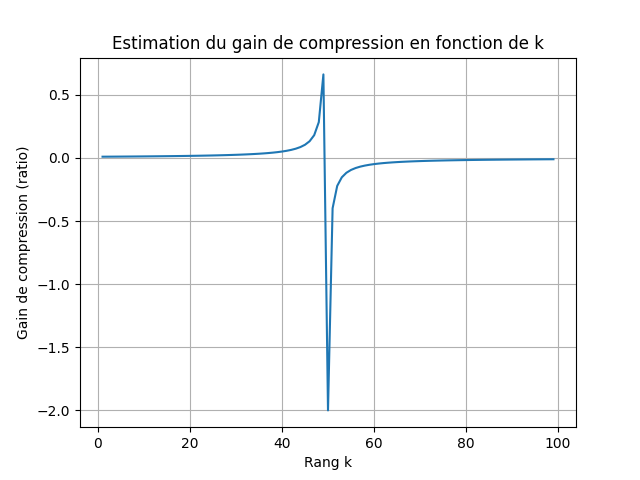
\includegraphics[width=\textwidth]{gain_estimation.png}
  \captionof{figure}{Estimation du gain de place en fonction de \( k \) pour une image de \( 100 \times 100 \).\\}
  \label{fig:gain_estimation}
\end{minipage}
\hfill
\begin{minipage}{0.62\textwidth}
Nous pouvons déjà estimer le gain de place obtenu en fonction de \( k \) pour une image ( matrice \( A \)) de taille \( m \times n \). Après compression, nous obtenons une approximation  $A' = U_k S_k V_k^T$, où $U_k$ et $V_k$ sont des matrices de taille $m \times k$ et $n \times k$, et $S_k$ est une matrice diagonale de taille $k \times k$ (mais nous ne stockons que les valeurs diagonales donc $k$ valeurs). \\
Le nombre total de valeurs stockées après compression est donc de \( k(m + n + 1)\) ce qui donne un gain de place de \( mn - k(m + n + 1) \). Pour que la compression soit efficace, il faut que ce gain soit strictement positif, c'est-à-dire que \( mn - k(m + n + 1) > 0 \) ou encore \( k < \frac{mn}{m + n + 1} \).
\end{minipage}
La figure \ref{fig:gain_estimation} montre que suivant les fourmules précédemment énoncé, le gain de place augmente de manière logarithmique avec \( k \). Pour une image de taille \( 100 \times 100 \) elle atteind un plateau $k > \frac{mn}{m + n + 1} = 50$ où le gain de place est maximal pour devenir négatif ce qui représente une augmentation de la taille de l'image compressée par rapport à l'originale.\\


\section{Résultats et discussions}
Dans cette section, nous présentons les résultats de nos expérimentations et discutons de la performance de nos algorithmes.

\subsection{Bidiagonalisation}
La comparaison des transformations de Householder appliquées via un produit usuel et par un produit de vecteurs, visible dans la figure \ref{fig:performance_comparison}, montre que la méthode par vecteurs est plus rapide que la méthode usuelle sur des matrices de tailles relatives à celles que nous manipulons pour notre utilisation. Néanmoins, la croissance du temps de calcul de la méthode par vecteurs pourrait s'avérer plus élevée pour des matrices de tailles plus grandes.\\
\begin{minipage}{0.37\textwidth}
  Les erreurs relatives quant à elles, bien que faibles (de l'ordre de $10^{-16}$), semblent croître linéairement pour notre méthode par vecteurs contrairement à la méthode usuelle qui semble avoir une erreur constante malgré des fluctuations à intervalles réguliers.\\ \\
  Le choix entre les deux méthodes dépendra donc de la taille des matrices que nous manipulons et de la précision que nous souhaitons obtenir. Ici, la méthode par vecteurs semble plus adaptée à notre utilisation.
  \end{minipage}
\hfill
\begin{minipage}{0.6\textwidth}
  \centering
  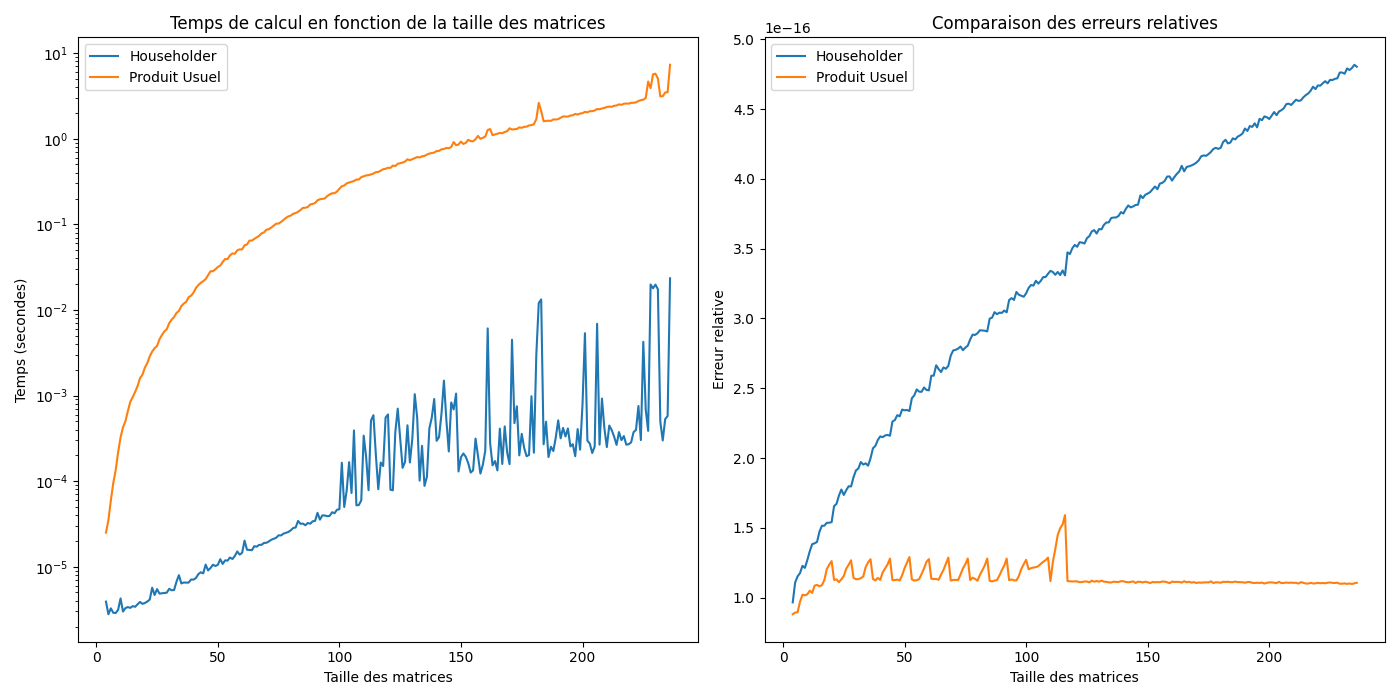
\includegraphics[width=\textwidth, trim=0.5cm 0 0 0, clip]{householder_comparaison.png}
  \captionof{figure}{Comparaison des performances entre le produit par vecteurs et le produit matriciel usuel par $H$ en fonction de la taille des matrices.}
  \label{fig:performance_comparison}
\end{minipage}

% \begin{minipage}{0.4\textwidth}
%   \centering
%   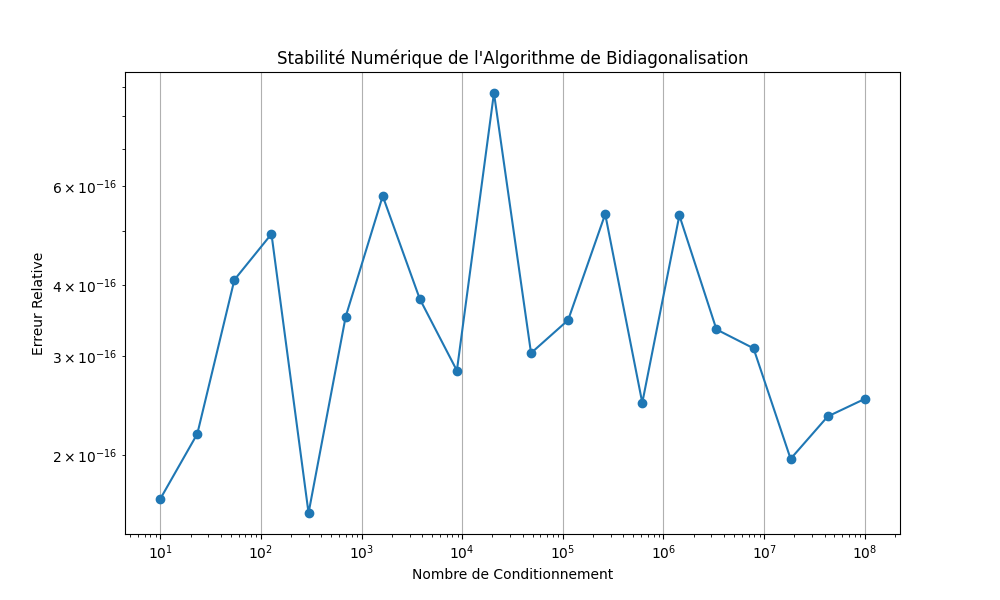
\includegraphics[width=\linewidth, trim=0.5cm 0 2.5cm 0, clip]{numeric_stability_bd.png}
%   \captionof{figure}{Stabilité numérique de l'algorithme de bidiagonalisation.}
%   \label{fig:stabilite}
% \end{minipage}
% \hfill
% \begin{minipage}{0.55\textwidth}
% L'analyse de la stabilité numérique de l'algorithme de bidiagonalisation~\ref{fig:stabilite} montre que l'erreur relative reste faible, de l'ordre de $10^{-16}$, même pour des nombres de conditionnement élevés allant jusqu'à $10^8$. Cela indique que l'algorithme est globalement stable numériquement, bien que des fluctuations mineures soient observées pour certaines matrices spécifiques.
% \end{minipage}

\subsection{Diagonalisation}
Nos différentes expérimentations sur la factorisation QR présentées dans la figure \ref{fig:performance_comparison_qr} montrent que notre méthode par rotations de Givens est plus rapide que notre implémentation de la méthode par Householder mais plus lente que la méthode de Numpy. Ce qui s'explique par le fait que la méthode de Numpy est optimisée par des calculs en C et par l'utilisation de la bibliothèque BLAS.\\ \\
\begin{minipage}{0.6\textwidth}
  \centering
  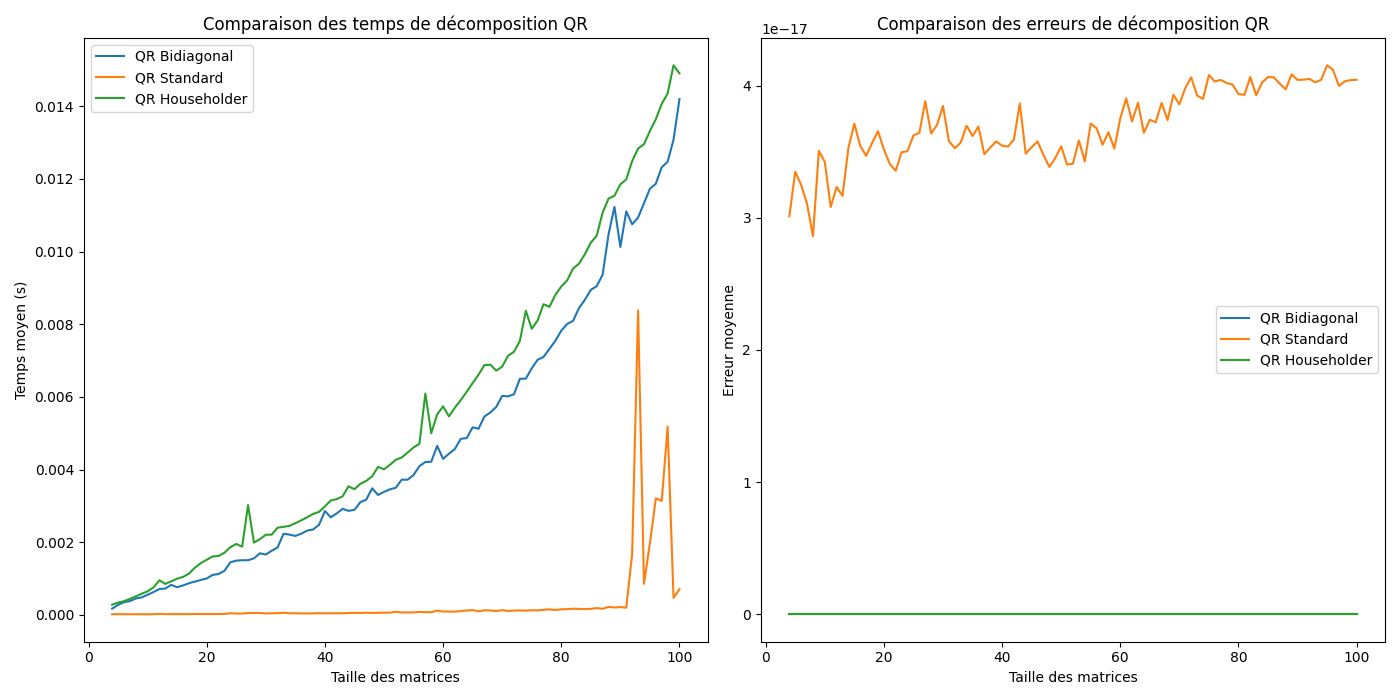
\includegraphics[width=\textwidth]{qr_comparaison.png}
  \captionof{figure}{Comparaison des performances de QR Householder, Numpy et par rotations de Givens en fonction de la taille des matrices.\\}
  \label{fig:performance_comparison_qr}
\end{minipage}
\hfill
\begin{minipage}{0.37\textwidth}
Cependant, on observe que la méthode par rotations de Givens est plus précise que Householder, bien que toutes deux restent très précises.\\
Les hauts pics de temps de calcul pour la méthode de Numpy qui apparaissent sur les matrices de taille plus grande pour des raisons que nous n'avons pas réussi à expliquer ont néanmoins eu un impact significatif sur les performances de nos algorithmes nous poussant à privilégier la méthode par rotations de Givens.
\end{minipage}
L'analyse de la convergence de la matrice S construite au cours de la SVD vers une matrice diagonale montre que celle-ci converge très rapidement, la norme des éléments extra diagonaux diminuant de manière exponentielle vers 0 au cours des itérations, comme l'illustre la figure \ref{fig:convergenceSVD}.
Leur quantité quant à elle décroît aussi très vite mais de manière linéaire, démontrant une quantité élevée d'éléments extra-diagonaux très peu significatifs.\\
\begin{minipage}{0.55\textwidth}
  \centering
  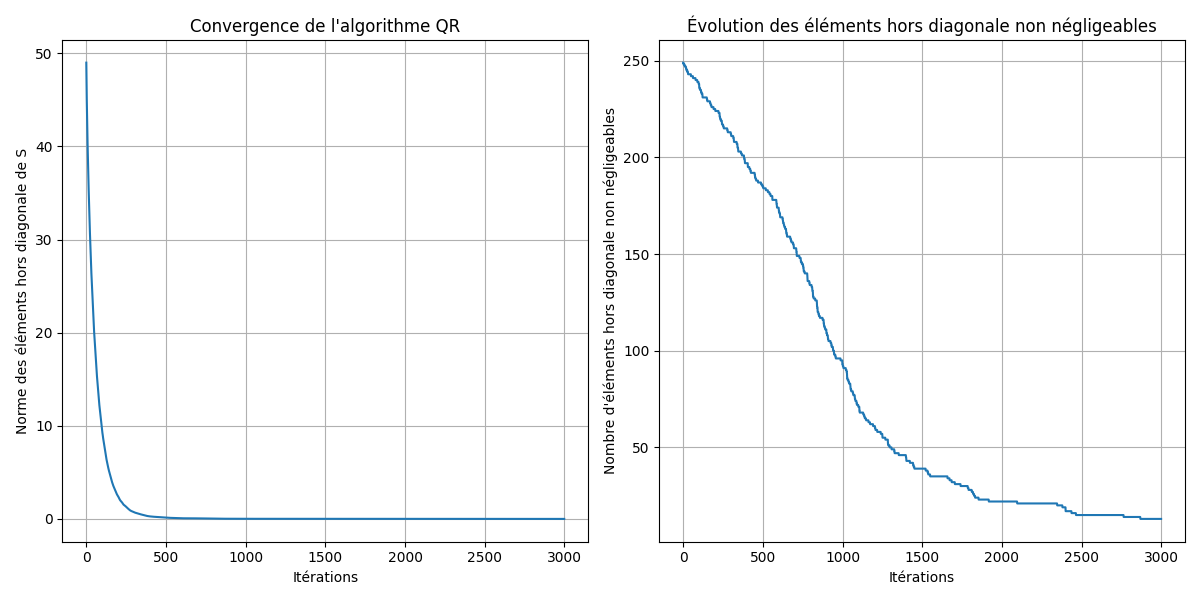
\includegraphics[width=\textwidth]{svd_convergence.png}
  \captionof{figure}{Évolution de la quantité et de la norme des éléments extra diagonaux selon le nombre d'itérations.\\}
  \label{fig:convergenceSVD}
\end{minipage}
\hfill
\begin{minipage}{0.4\textwidth}
  \centering
  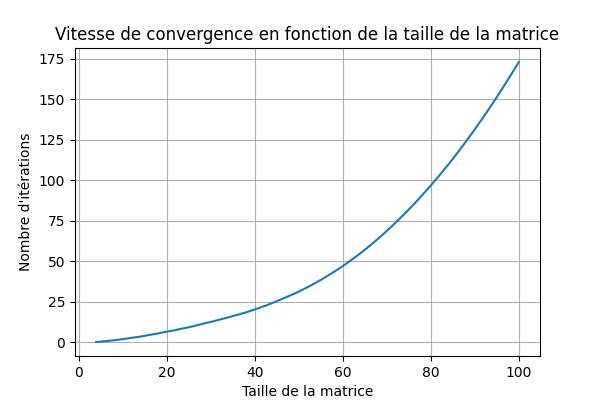
\includegraphics[width=\textwidth]{svd_convergence_size.png}
  \captionof{figure}{Nombre d'itérations nécessaires pour atteindre un seuil de convergence en fonction de la taille de la matrice.\\}
  \label{fig:sizeSVD}
\end{minipage}
\\ La figure \ref{fig:sizeSVD} démontre quant à elle que pour un seuil de convergence donné, le nombre d'itérations nécessaires avant de l'atteindre augmente quadratiquement selon la taille de la matrice. Ce qui est cohérent avec la complexité en $O(n^2)$ de notre algorithme.\\
Grâce à ces résultats, nous pouvons mieux ajuster notre paramètre de convergence pour obtenir un bon compromis entre précision et temps de calcul.

\subsection{Application à la compression d'images}
En appliquant notre algorithme de SVD à la compression d'images, nous avons pu obtenir différents seuils de compression altérant plus ou moins la qualité de l'image, comme le représente la figure \ref{fig:comparison}. Ici, la compression appliquée est celle par canaux séparés, mais aucune différence visuelle n'est notable entre les deux méthodes.
\begin{figure}[H]
    \centering
    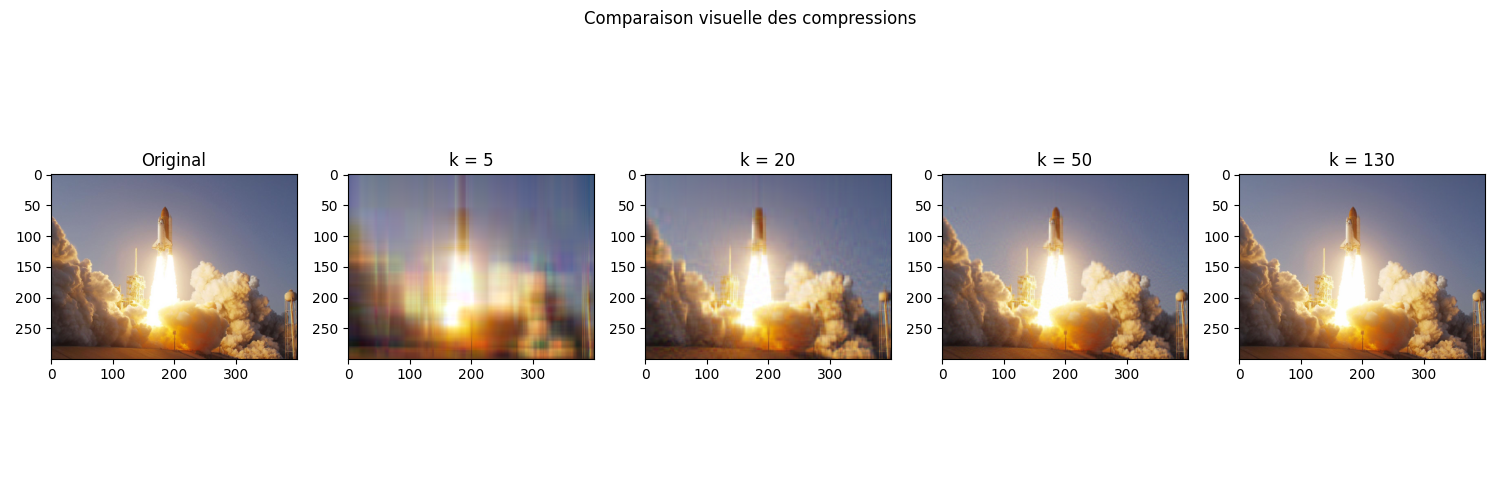
\includegraphics[width=\textwidth, trim=0 3cm 0 3.7cm, clip]{comparison.png}
    \caption{De gauche à droite : image originale, et image compressée avec \( k \), allant de 5 à 130 (méthode par canaux séparés). \textit{Source : Domaine public Nasa}}
    \label{fig:comparison}
\end{figure}
On observe néanmoins que l'impact sur la qualité visuelle de l'image semble suivre une courbe logarithmique, les premières valeurs singulières étant les plus significatives. Observation confirmée par la figure \ref{fig:error_gain_plot} qui montre que l'erreur de reconstruction diminue de manière logarithmique avec \( k \) tandis que le gain de place augmente de manière linéaire quelque soit la méthode de compression utilisée, ce qui est en contradiction avec notre estimation théorique, nous poussant à revoir notre formule et nos implémentations.
\begin{figure}[H]
  \centering
  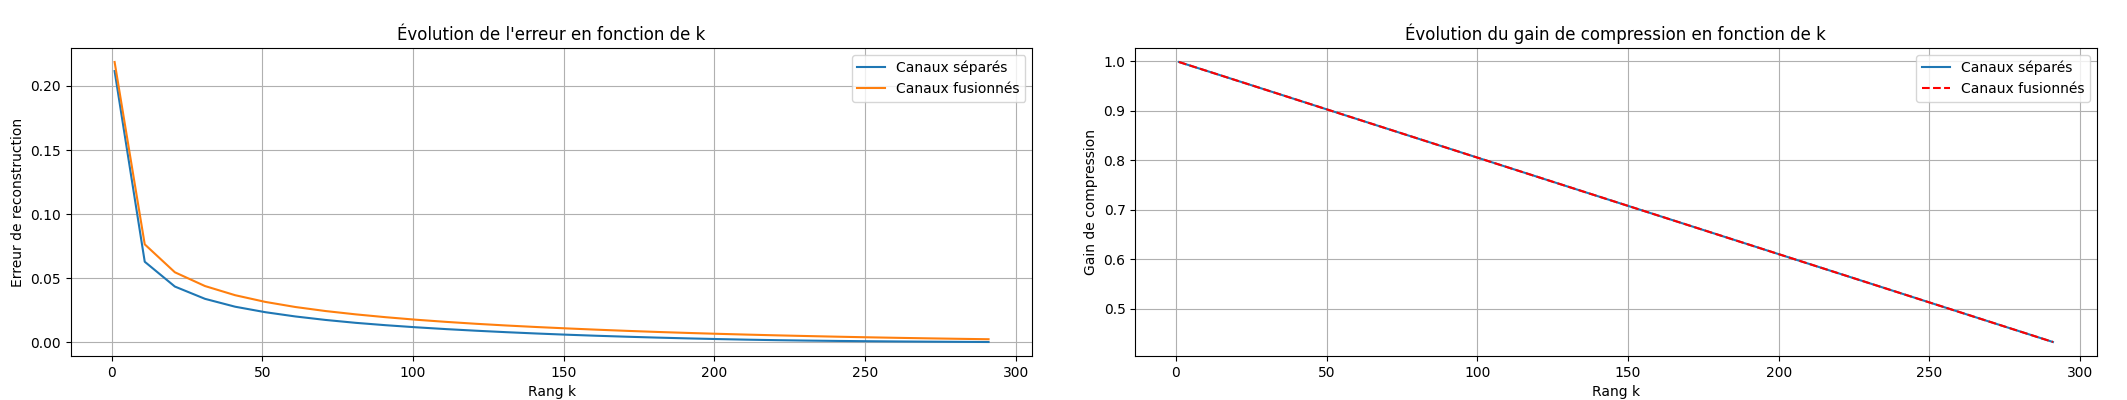
\includegraphics[width=\textwidth]{error_gain_plot2.png}
  \caption{Évolution du gain de place et de l'erreur en fonction du rang \( k \).}
  \label{fig:error_gain_plot}
\end{figure}
La figure \ref{fig:error_gain_plot} montre aussi que la méthode par canaux séparés est légèrement plus efficace que la méthode par fusion des canaux de couleur pour des valeurs de \( k \) faibles, mais que la différence de performances s'atténue pour des valeurs de \( k \) plus élevées. Le gain quant à lui est évidemment le même quelle que soit la méthode utilisée.\\

\begin{minipage}{0.45\textwidth}
  \centering
  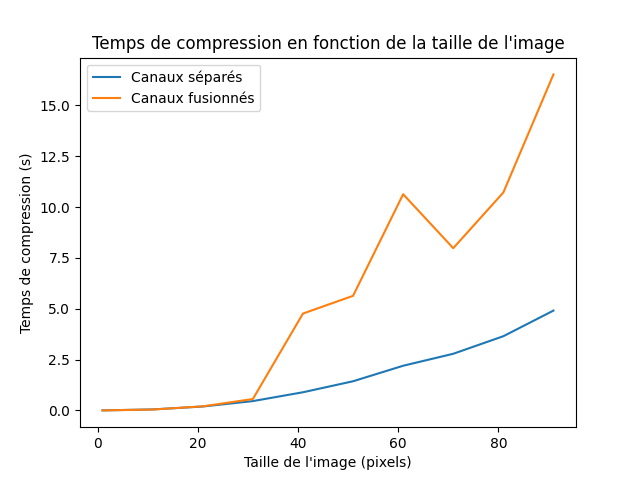
\includegraphics[width=\textwidth]{time_plot.png}
  \captionof{figure}{Temps de calcul en fonction de la taille de l'image pour \( k = 5 \).\\}
  \label{fig:time_plot}
\end{minipage}
\hfill
\begin{minipage}{0.5\textwidth}
  La figure~\ref{fig:time_plot} montre que le temps de calcul de notre algorithme de compression d'image par canaux séparés est linéaire en fonction de la taille de l'image alors que le temps de calcul de la méthode par fusion des canaux de couleur croît rapidement par paliers.\\
  Cela est dû au fait que la méthode par fusion des canaux de couleur nécessite de manipuler des matrices de taille plus grande que la méthode par canaux séparés et nous avons vu précédemment que la complexité de notre algorithme de SVD est en $O(n^2)$. Le temps de compression par canaux séparés sera donc $O(3n^2)$ tandis que celui par fusion des canaux de couleur sera $O(9n^2)$.
\end{minipage}


% \section{Conclusion et perspectives}
% Dans ce projet, nous avons développé un algorithme de compression d'images basé sur la factorisation SVD. Nous avons implémenté des transformations de Householder pour bidiagonaliser les matrices, puis utilisé une décomposition QR itérative pour obtenir la SVD. Les résultats montrent une compression efficace avec une perte minimale d'information visuelle.\\
% Nos expérimentations ont montré que la méthode par rotations de Givens est plus rapide et plus précise que la méthode par Householder. Nous avons aussi observé que la méthode par canaux séparés est plus efficace que la méthode par fusion des canaux de couleur en temps et en précison.\\
% Pour aller plus loin, il serait intéressant d'explorer d'autres méthodes de compression d'images basées sur la factorisation SVD, telles que la compression par blocs ou la compression par ondelettes. Il serait également intéressant d'optimiser davantage nos algorithmes pour les rendre plus rapides et plus précis.
\end{document}